\documentclass[aspectratio=169,10pt]{beamer}
\usetheme{metropolis}
\usepackage{booktabs}
\usepackage{graphicx}
\usepackage{amsmath}
\usepackage{xcolor}
\usepackage{tikz}
\usepackage{adjustbox}
\usetikzlibrary{arrows.meta,positioning}

\definecolor{good}{RGB}{39,174,96}
\definecolor{warn}{RGB}{192,57,43}
\definecolor{muted}{RGB}{120,120,120}
\definecolor{accent}{RGB}{46,106,178}

\setbeamertemplate{footline}{%
  \hfill\insertframenumber/\inserttotalframenumber\hspace*{1em}\vspace*{0.5em}}

\title{EB-JEPA for Clinical EEG}
\subtitle{Self-Supervised Abnormality Detection}
\author{Timothy Courtois \and Théo Basséras \and Yani Hammache \and Titouan Vasnier}
\date{Hackathon, June 2026}

\begin{document}
\maketitle

\begin{frame}{Why Self-Supervised EEG?}
\begin{columns}[T]
\column{0.55\textwidth}
\textbf{Clinical reality:}
\begin{itemize}\setlength\itemsep{0pt}
  \item Every EEG must be reviewed by a licensed neurologist
  \item Labels are scarce and expensive
  \item Unlabelled EEG data is abundant
\end{itemize}

\vspace{0.3em}
\textbf{Goal:} learn a \emph{transferable} EEG representation \textbf{without labels}

\vspace{0.3em}
\textbf{Hypothesis:} corruption augmentation + weak invariance ($\lambda{=}1$) is the dominant lever, not encoder scale.

\vspace{0.3em}
\textbf{Benchmark: TUAB v3.0.1}
\begin{itemize}\setlength\itemsep{0pt}
  \item Binary: normal / abnormal clinical EEG
  \item 19 channels, 200\,Hz, 10\,s windows
  \item 2\,717 train / 276 eval (patient-disjoint)
\end{itemize}

\column{0.42\textwidth}
\begin{center}
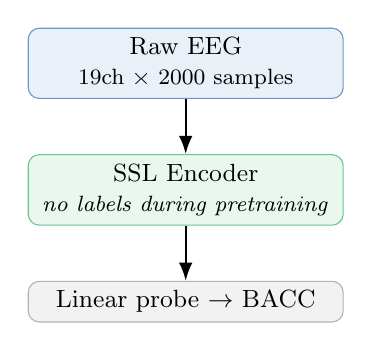
\begin{tikzpicture}[font=\small, node distance=0.7cm]
  \node[draw=accent!70, fill=accent!10, rounded corners, minimum width=4cm, align=center]
    (raw) {Raw EEG\\ \footnotesize 19ch × 2000 samples};
  \node[draw=good!70, fill=good!10, rounded corners, below=of raw, minimum width=4cm, align=center]
    (enc) {SSL Encoder\\ \footnotesize \emph{no labels during pretraining}};
  \node[draw=gray!60, fill=gray!10, rounded corners, below=of enc, minimum width=4cm, align=center]
    (probe) {Linear probe $\to$ BACC};
  \draw[-{Latex}, thick] (raw) -- (enc);
  \draw[-{Latex}, thick] (enc) -- (probe);
\end{tikzpicture}
\end{center}
\end{columns}
\end{frame}

\begin{frame}{Plato's Cave: What SSL Actually Does}
\begin{columns}[T]
\column{0.55\textwidth}
Prisoners in Plato's cave see only \textbf{shadows on the wall}, not the real objects. They learn to \emph{predict} patterns in the shadows without ever seeing the cause.

\vspace{0.4em}
\textbf{In our setting:}
\begin{itemize}\setlength\itemsep{0pt}
  \item Cave wall = raw EEG voltages
  \item Hidden reality = underlying brain pathology
  \item SSL encoder = prisoner learning that \emph{two corrupted views of the same shadow are the same object}
  \item Linear probe = asking the prisoner to name what they see
\end{itemize}

\vspace{0.2em}
\textcolor{muted}{\footnotesize The encoder never sees a neurologist's label. It learns structure from the signal alone.}

\column{0.42\textwidth}
\begin{center}
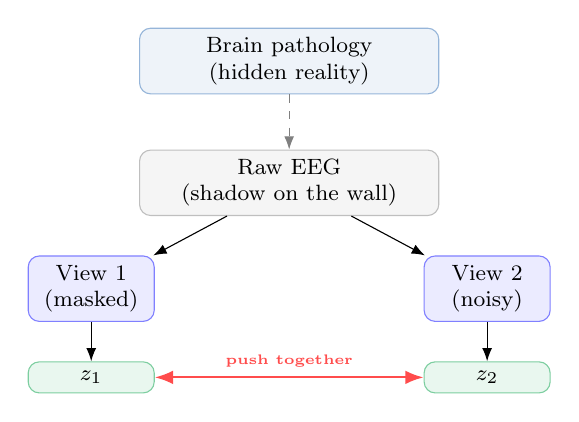
\begin{tikzpicture}[font=\footnotesize, node distance=0.5cm and 0.5cm]
  \node[draw=accent!50, fill=accent!8, rounded corners, minimum width=3.8cm, align=center]
    (brain) {Brain pathology\\ \footnotesize (hidden reality)};
  \node[draw=gray!50, fill=gray!8, rounded corners, below=0.7cm of brain, minimum width=3.8cm, align=center]
    (eeg) {Raw EEG\\ \footnotesize (shadow on the wall)};
  \node[draw=blue!50, fill=blue!8, rounded corners, below left=0.5cm and -0.2cm of eeg, minimum width=1.6cm, align=center]
    (v1) {View 1\\ \footnotesize (masked)};
  \node[draw=blue!50, fill=blue!8, rounded corners, below right=0.5cm and -0.2cm of eeg, minimum width=1.6cm, align=center]
    (v2) {View 2\\ \footnotesize (noisy)};
  \node[draw=good!60, fill=good!10, rounded corners, below=0.5cm of v1, minimum width=1.6cm, align=center]
    (z1) {$z_1$};
  \node[draw=good!60, fill=good!10, rounded corners, below=0.5cm of v2, minimum width=1.6cm, align=center]
    (z2) {$z_2$};
  \draw[-{Latex},dashed,gray] (brain) -- (eeg);
  \draw[-{Latex}] (eeg) -- (v1); \draw[-{Latex}] (eeg) -- (v2);
  \draw[-{Latex}] (v1) -- (z1); \draw[-{Latex}] (v2) -- (z2);
  \draw[{Latex}-{Latex}, red!70, thick] (z1.east) -- (z2.west)
    node[midway,above,font=\tiny\bfseries,text=red!70]{push together};
\end{tikzpicture}
\end{center}
\end{columns}
\end{frame}

\begin{frame}{EB-JEPA: Two-View Invariance + Corruption}
\begin{columns}[T]
\column{0.55\textwidth}
\textbf{Two-view SSL pipeline:}
\begin{enumerate}\setlength\itemsep{0pt}
  \item Take one EEG window; create two views $v_1, v_2$
  \item Encode: $z_i = f_\theta(v_i) \in \mathbb{R}^{256}$
  \item Minimise $\|z_1 - z_2\|^2$ + anti-collapse term
\end{enumerate}

\vspace{0.2em}
\textbf{Standard augmentations:} noise, jitter, channel drop

\vspace{0.2em}
\textbf{Our design: Corruption augmentation}
\begin{itemize}\setlength\itemsep{0pt}
  \item 20\,\% time steps \textbf{masked} to zero
  \item 20\,\% time steps injected with $\pm6\sigma$ \textbf{spikes}
  \item Mimics real EEG artefacts; forces robust learning
\end{itemize}

\vspace{0.2em}
\textbf{Objectives:} VICReg ($V$+$C$) and SIGReg (Epps-Pulley)

\column{0.42\textwidth}
\begin{center}
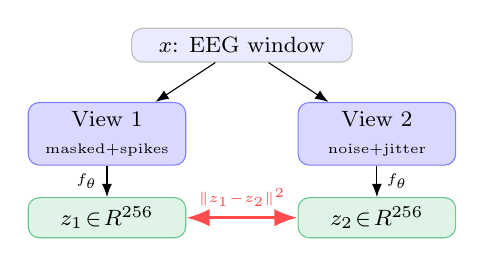
\begin{tikzpicture}[font=\footnotesize, node distance=0.5cm and 0.5cm]
  \node[draw=gray!50, fill=blue!8, rounded corners, minimum width=2.8cm, align=center]
    (x) {$x$: EEG window};
  \node[draw=blue!50, fill=blue!15, rounded corners, below left=0.5cm and -0.7cm of x, minimum width=2.0cm, align=center]
    (v1) {View 1\\ \tiny masked+spikes};
  \node[draw=blue!50, fill=blue!15, rounded corners, below right=0.5cm and -0.7cm of x, minimum width=2.0cm, align=center]
    (v2) {View 2\\ \tiny noise+jitter};
  \node[draw=good!70, fill=good!15, rounded corners, below=0.4cm of v1, minimum width=2.0cm, align=center]
    (z1) {$z_1\!\in\!\mathbb{R}^{256}$};
  \node[draw=good!70, fill=good!15, rounded corners, below=0.4cm of v2, minimum width=2.0cm, align=center]
    (z2) {$z_2\!\in\!\mathbb{R}^{256}$};
  \draw[-{Latex}] (x) -- (v1); \draw[-{Latex}] (x) -- (v2);
  \draw[-{Latex}] (v1) -- (z1) node[midway,left,font=\tiny]{$f_\theta$};
  \draw[-{Latex}] (v2) -- (z2) node[midway,right,font=\tiny]{$f_\theta$};
  \draw[{Latex}-{Latex}, red!70, very thick] (z1.east) -- (z2.west)
    node[midway, above, font=\tiny\bfseries, text=red!70]{$\|z_1{-}z_2\|^2$};
\end{tikzpicture}
\end{center}
\end{columns}
\end{frame}

\begin{frame}{Finding 1: Corruption Augmentation as Dominant Lever}
\begin{columns}[T]
\column{0.55\textwidth}
{\scriptsize
\begin{tabular}{p{3.5cm}cc}
\toprule
Variant & BACC\textsubscript{REC} & $\Delta$ \\
\midrule
Base VICReg (no corruption) & 0.796 & -- \\
\textbf{+ Corruption} (3-seed) & \textbf{0.819±.004} & \textcolor{good}{+0.023} \\
\textbf{+ spectral} (best run) & \textbf{0.836} & \textcolor{good}{+0.040} \\
+ spectral + stylised-facts & 0.823±.007 & $\approx$0 \\
1.35M conv (3-seed) & 0.812±.021 & $-$0.007 \\
25\% pretraining data & 0.816 & $-$0.008 \\
\bottomrule
\end{tabular}
}

\vspace{0.5em}
\textbf{3-seed robust avg:} $0.819 \pm 0.004$ (corruption only); single best run w/ spectral loss: 0.836.

\column{0.42\textwidth}
\textbf{Why corruption helps:}
\begin{itemize}
  \item Standard augmentation creates views that are ``too easy'' to match
  \item Masking + spike injection forces learning \emph{content}, not artefact patterns
  \item Mirrors real EEG noise distribution
\end{itemize}

\vspace{0.5em}
\textbf{What does NOT help:}
\begin{itemize}
  \item Scaling 0.4M $\to$ 1.35M params → same plateau
  \item 4$\times$ less pretraining data costs only 0.8\,pp → not data-starved
  \item Piling stylised-facts terms on top of spectral → flat
  \item[$\Rightarrow$] Bottleneck is \emph{architecture}, not scale or data
\end{itemize}
\end{columns}
\end{frame}

\begin{frame}{Finding 2 (Novel): EEG Prefers Weak VICReg Invariance}
\begin{columns}[T]
\column{0.55\textwidth}
\textbf{VICReg loss:}
\[
\mathcal{L} = \lambda_{\rm inv}\underbrace{\|z_1{-}z_2\|^2}_{\text{inv}}
             + 25\,V + 1\,C
\]
Paper-correct: $\lambda_{\rm inv} = 25$. Default: $\lambda_{\rm inv} = 1$.

\vspace{0.3em}
{\small
\begin{tabular}{lcc}
\toprule
$\lambda_{\rm inv}$ & BACC\textsubscript{REC} & Seeds \\
\midrule
1 (default)  & \textbf{0.819 ± .004} & 3 \\
5            & 0.820               & 1 \\
10           & 0.814               & 1 \\
25 (paper)   & 0.789 ± .005       & 3 \\
\midrule
\multicolumn{3}{l}{\footnotesize Gap $\lambda{=}1$ vs $\lambda{=}25$: 3\,pp, ${\approx}6\sigma$, not noise}
\end{tabular}
}

\column{0.42\textwidth}
\textbf{Why?}
\begin{itemize}\setlength\itemsep{0pt}
  \item With $\lambda{=}1$: anti-collapse ($V$+$C$) \textbf{dominates}
  \item Encoder spreads representations: more discriminative
  \item With $\lambda{=}25$: encoder collapses toward view-similarity
\end{itemize}

\vspace{0.3em}
\textbf{Sweep $\lambda \in \{1,5,10,25\}$:}
Sweet spot at $\{1,5\}$; gap widens monotonically.

\vspace{0.3em}
\textcolor{accent}{\footnotesize First evidence that EEG SSL requires weaker view-invariance than vision SSL.
Confirmed on a second, independent 1.35M+spectral config: $1(0.824){>}5(0.820){>}10(0.814){>}25(0.804)$, same monotone order.}
\end{columns}
\end{frame}

\begin{frame}{NaiveJEPA: Temporal-Split Prediction, No Anti-Collapse Needed}
\begin{columns}[T]
\column{0.55\textwidth}
\textbf{Idea}: split one window in time instead of augmenting.

\vspace{0.4em}
\begin{itemize}
  \item Context ($0\to T/2$): online encoder $\to$ mean-pool
  \item Target ($T/2\to T$): EMA encoder $\to$ mean-pool
  \item Loss: $\mathrm{MSE}(\hat{z}_{\rm tgt},\ z_{\rm tgt})$
  \item \textbf{No VICReg needed:} collapse resisted by BatchNorm (zero variance $\to$ explosion) + EMA lag (non-stationary target)
\end{itemize}

\vspace{0.4em}
{\small
\begin{tabular}{lcc}
\toprule
Method & BACC\textsubscript{REC} & Hypers \\
\midrule
VICReg + corruption & 0.819 ± .004 & 4 \\
\textbf{NaiveJEPA}  & \textbf{0.779}        & \textbf{1} \\
\bottomrule
\end{tabular}
}

\column{0.42\textwidth}
\begin{center}
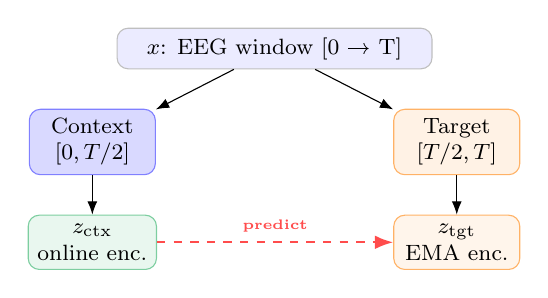
\begin{tikzpicture}[font=\footnotesize, node distance=0.5cm and 0.5cm]
  \node[draw=gray!50, fill=blue!8, rounded corners, minimum width=4cm, align=center]
    (x) {$x$: EEG window [0 → T]};
  \node[draw=blue!50, fill=blue!15, rounded corners, below left=0.5cm and -0.5cm of x,
        minimum width=1.6cm, align=center]
    (ctx) {Context\\ $[0, T/2]$};
  \node[draw=orange!60, fill=orange!10, rounded corners, below right=0.5cm and -0.5cm of x,
        minimum width=1.6cm, align=center]
    (tgt) {Target\\ $[T/2, T]$};
  \node[draw=good!60, fill=good!10, rounded corners, below=0.5cm of ctx, minimum width=1.6cm, align=center]
    (zc) {$z_{\rm ctx}$\\ online enc.};
  \node[draw=orange!60, fill=orange!8, rounded corners, below=0.5cm of tgt, minimum width=1.6cm, align=center]
    (zt) {$z_{\rm tgt}$\\ EMA enc.};
  \draw[-{Latex}] (x) -- (ctx); \draw[-{Latex}] (x) -- (tgt);
  \draw[-{Latex}] (ctx) -- (zc); \draw[-{Latex}] (tgt) -- (zt);
  \draw[-{Latex}, red!70, thick, dashed] (zc.east) -- (zt.west)
    node[midway,above,font=\tiny\bfseries,text=red!70]{predict};
\end{tikzpicture}
\end{center}

\vspace{0.3em}
\textcolor{muted}{\footnotesize 0.04 BACC below VICReg+corruption, with 1 hyperparameter.}
\end{columns}
\end{frame}

\begin{frame}{Encoder Ranking: Simple Conv Wins}
\begin{columns}[T]
\column{0.50\textwidth}
\textbf{Validated, bug-free (capacity-matched, BACC):}
{\scriptsize
\begin{tabular}{lccc}
\toprule
Encoder & Type & Params & BACC\textsubscript{REC} \\
\midrule
\textcolor{good}{\textbf{Conv1D}} & Strided & 1.35M & \textbf{0.824} \\
Transformer & Scratch & 1.29M & \textcolor{warn}{0.725 ($-$10pp)} \\
\bottomrule
\end{tabular}
}

\vspace{0.4em}
{\footnotesize\textcolor{muted}{Early exploration (pre-bugfix VICReg coeffs, raw accuracy not BACC) had
also flagged LaBraM-/BIOT-style patch transformers ($\sim$0.78--0.84 acc) and EEGPT (below-random-floor
collapse) as weaker than conv --- directionally consistent with the validated result above, but not
re-measured post-fix.}}

\vspace{0.3em}
\textbf{EEGPT failure (confirmed, post-fix):} cross-attention pools 19\,ch $\to$ 1 token; channel-drop creates incompatible views.
Fix: remove channel-drop $\to$ TUEV 0.182 $\to$ 0.358.

\column{0.48\textwidth}
\IfFileExists{figures/encoder_comparison.png}{%
  \includegraphics[width=\linewidth]{figures/encoder_comparison.png}
}{%
  \begin{center}\textcolor{muted}{\footnotesize [encoder comparison figure]}\end{center}
}
\end{columns}
\end{frame}

\begin{frame}{Position vs Literature}

{\small
\textbf{Evaluation trap:} literature (BIOT, LaBraM) reports \textbf{per-window} BACC.
Our setup mean-pools 16 windows/patient $\to$ \textbf{per-recording} ($+5$\,pp for same encoder).
Direct comparison manufactures a false win.
}

\vspace{0.2em}
\begin{columns}[T]
\column{0.50\textwidth}
{\small
\begin{tabular}{lcc}
\toprule
Method & BACC\textsubscript{WIN} & AUROC \\
\midrule
\textcolor{muted}{ContraWR (SSL)}      & \textcolor{muted}{0.775} & \textcolor{muted}{0.846} \\
\textcolor{accent}{BIOT pretrained}    & \textcolor{accent}{0.802} & \textcolor{accent}{0.874} \\
\textcolor{accent}{LaBraM-Base}        & \textcolor{accent}{0.814} & \textcolor{accent}{0.902} \\
\midrule
\textbf{EB-JEPA SIGReg+corrupt}        & \textbf{0.775} & \textbf{0.856} \\
EB-JEPA VICReg+corrupt                 & 0.770 & 0.848 \\
EEGNet (supervised)                    & 0.796 & 0.882 \\
\bottomrule
\end{tabular}
}
\vspace{0.2em}

\textcolor{good}{$\checkmark$} Matches ContraWR (1.6M) with 0.4M params\\
\textcolor{warn}{$\times$} 3.9\,pp below LaBraM (5.8M, 200 ep)

\column{0.48\textwidth}
\IfFileExists{figures/summary_vs_baselines.png}{%
  \includegraphics[width=\linewidth]{figures/summary_vs_baselines.png}
}{%
  \begin{center}\textcolor{muted}{\footnotesize [summary vs baselines figure]}\end{center}
}
\end{columns}
\end{frame}

\begin{frame}{Cross-Task Transfer to TUEV (6-class Event Detection)}
\begin{columns}[T]
\column{0.55\textwidth}
\textbf{Protocol}: freeze TUAB-pretrained encoder; train linear probe on TUEV (zero TUEV labels during SSL).

\vspace{0.4em}
{\scriptsize
\begin{tabular}{p{3.6cm}cc}
\toprule
Method & TUEV BACC & Labels? \\
\midrule
ST-Transformer  & 0.3385 & \textcolor{warn}{full train} \\
CNN-Transformer & 0.4100 & \textcolor{warn}{full train} \\
\midrule
VICReg+corrupt (TUAB SSL) & 0.382 & \textcolor{good}{probe only} \\
NaiveJEPA (TUAB SSL) & 0.389 & \textcolor{good}{probe only} \\
\textbf{+spectral} (best) & \textbf{0.425} & \textcolor{good}{probe only} \\
\midrule
FFCL            & 0.4551 & \textcolor{warn}{full train} \\
ContraWR        & 0.4664 & \textcolor{warn}{full train} \\
BIOT pretrained & 0.5009 & \textcolor{warn}{full train} \\
\bottomrule
\end{tabular}
}

\column{0.42\textwidth}
Zero TUEV labels seen during SSL pretraining.
A linear probe on frozen features beats \textbf{ST-Transformer} and \textbf{CNN-Transformer} trained end-to-end on TUEV.

\vspace{0.5em}
\textcolor{accent}{\small Transfer from a binary task to a 6-class task with only logistic regression: strongest evidence of genuine generality.}

\vspace{0.5em}
\textcolor{muted}{\footnotesize We trail BIOT/ContraWR/FFCL because they fine-tune or train from scratch on TUEV.}
\end{columns}
\end{frame}

\begin{frame}{Latent Space: EB-JEPA Representations}
\begin{columns}[T]
\column{0.74\textwidth}
\IfFileExists{figures/comparison_4methods_lda_honest.png}{%
  \includegraphics[width=\linewidth]{figures/comparison_4methods_lda_honest.png}
}{%
  \begin{center}\textcolor{muted}{\footnotesize [figure pending]}\end{center}
}
\column{0.24\textwidth}
{\small
\textbf{Setup:} Conv1D + VICReg $\lambda{=}1$ + corruption (BACC 0.819). 276 eval patients, 256-dim.

\vspace{0.3em}
\textbf{PCA/UMAP/t-SNE} look mixed. VICReg spreads signal across all 256 dims equally; 2D projections lose the discriminative direction. Expected, not a failure.

\vspace{0.3em}
\textbf{LDA} (4th): fit on \emph{train} (2717), projected on \emph{eval} (honest). Near-clean separation confirms BACC 0.819 is real.

\vspace{0.2em}
\textcolor{muted}{\tiny Labels never used during pretraining.}
}
\end{columns}
\end{frame}

\begin{frame}{Latent Space: 3D UMAP (EB-JEPA, Window-Level)}
\begin{columns}[T]
\column{0.62\textwidth}
\IfFileExists{latent_viz/latent_umap3d_window_seed0_a0.png}{%
  \includegraphics[width=\linewidth]{latent_viz/latent_umap3d_window_seed0_a0.png}
}{%
  \begin{center}\textcolor{muted}{\footnotesize [figure pending]}\end{center}
}
\column{0.35\textwidth}
{\small
\textbf{Setup:} same encoder, window-level latents (seed 0), 3D UMAP instead of 2D.

\vspace{0.3em}
2\,400 normal / 2\,016 abnormal windows. The third dimension recovers a two-lobe structure that 2D UMAP collapses.

\vspace{0.3em}
\textcolor{muted}{\footnotesize Still unsupervised projection (no labels used to fit UMAP) — qualitative support for Finding 1, not the BACC evidence (that's LDA, previous slide).}
}
\end{columns}
\end{frame}

\begin{frame}{Latent Space: BIOT (LDA, Same Protocol)}

\begin{columns}[T]
\column{0.62\textwidth}
\begin{center}
{\small\textbf{BIOT pretrained}: EEG-SHHS+PREST-18ch}\\
{\footnotesize BACC\textsubscript{WIN} 0.802 (sleep+pathology pretraining, 1.2M)}
\end{center}
\IfFileExists{figures/lda_honest_biot.png}{%
  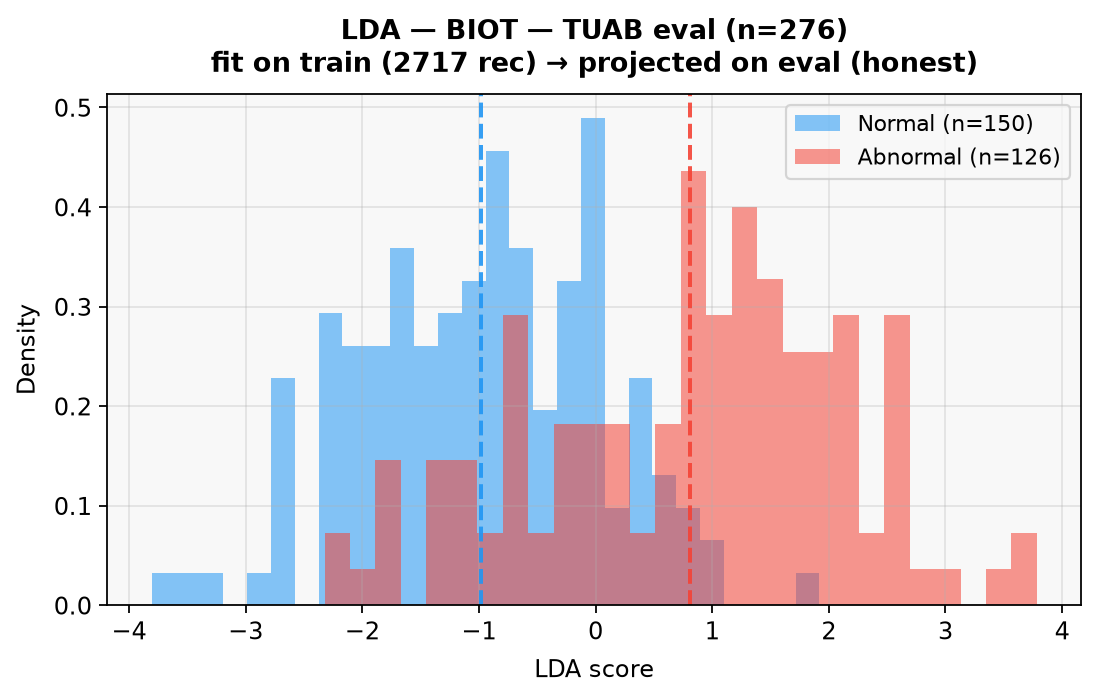
\includegraphics[width=\linewidth]{figures/lda_honest_biot.png}
}{%
  \begin{center}\textcolor{muted}{\footnotesize [figure pending]}\end{center}
}
\column{0.33\textwidth}
{\small
\textbf{Same LDA protocol} as EB-JEPA (slide before last): fit on TUAB \emph{train} (2717 rec), projected on \emph{eval} (276 rec, honest).

\vspace{0.3em}
EB-JEPA: BACC\textsubscript{REC} 0.819, 0.4M params.

\vspace{0.3em}
\textcolor{muted}{\footnotesize BIOT pretrained on sleep EEG (SHHS); domain mismatch with clinical pathology may reduce separability.}
}
\end{columns}
\end{frame}

\begin{frame}{Summary}

\begin{columns}[T]
\column{0.50\textwidth}
\textbf{\textcolor{good}{What works}}
\begin{itemize}
  \item \textbf{Corruption}: +2.3\,pp BACC (3-seed, robust)
  \item \textbf{$\lambda_{\rm inv}{=}1$}: beats $\lambda{=}25$ by 3\,pp/$6\sigma$, EEG-specific
  \item \textbf{SIGReg $\geq$ VICReg}: consistent +0.5--1\,pp AUROC
  \item \textbf{NaiveJEPA}: 0.779 BACC with 1 hyperparameter
  \item \textbf{TUEV transfer}: beats 2 supervised baselines, zero TUEV labels
\end{itemize}

\column{0.48\textwidth}
\textbf{\textcolor{warn}{What doesn't}}
\begin{itemize}
  \item Scaling the encoder (capacity is not the limit)
  \item 4$\times$ pretraining data (conv saturates)
  \item EEGPT (channel-drop × channel-pool conflict)
  \item Spectral auxiliary loss (neutral)
  \item GRU predictive JEPA (same-window degenerates)
\end{itemize}
\end{columns}

\vspace{0.5em}
\begin{block}{Open next step}
$\lambda_{\rm inv}$ sweep $\{1,5,10,25\}$ confirms monotone ordering: EEG SSL prefers weaker invariance, first systematic evidence in the literature.
\end{block}
\end{frame}

\begin{frame}{}
\vspace{1.5em}
\begin{center}
{\Huge\bfseries Thank you}\\[1em]
{\large\textcolor{muted}{EB-JEPA for Clinical EEG --- self-supervised, frozen, label-free pretraining}}\\[1.5em]
{\large Questions welcome}
\end{center}
\vspace{1em}
\begin{center}
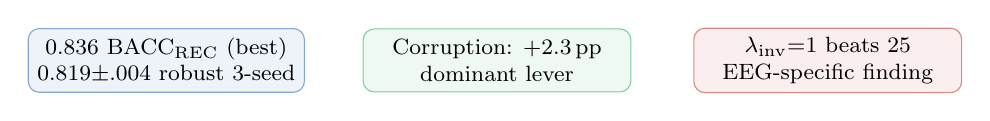
\begin{tikzpicture}[font=\footnotesize]
  \node[draw=accent!60, fill=accent!8, rounded corners, minimum width=3.4cm, align=center, minimum height=0.8cm]
    (a) at (0,0) {0.836 BACC\textsubscript{REC} (best)\\\footnotesize 0.819$\pm$.004 robust 3-seed};
  \node[draw=good!60, fill=good!8, rounded corners, minimum width=3.4cm, align=center, minimum height=0.8cm]
    (b) at (4.2,0) {Corruption: +2.3\,pp\\\footnotesize dominant lever};
  \node[draw=warn!60, fill=warn!8, rounded corners, minimum width=3.4cm, align=center, minimum height=0.8cm]
    (c) at (8.4,0) {$\lambda_{\rm inv}{=}1$ beats 25\\\footnotesize EEG-specific finding};
\end{tikzpicture}
\end{center}
\vspace{1em}
\begin{center}\textcolor{muted}{\footnotesize Backup slides follow: per-recording table, $\lambda_{\rm inv}$ ablation.}\end{center}
\end{frame}

\begin{frame}{Backup: Per-Recording Table (Clinical Metric)}
\small
\begin{tabular}{lccc}
\toprule
Model & BACC\textsubscript{REC} & AUROC & Eval \\
\midrule
Conv + VICReg + spectral 0.1 (best single run) & \textbf{0.836} & 0.887 & Frozen \\
Conv + VICReg + corruption (3 seeds) & 0.819 ± .004 & \textbf{0.900 ± .006} & Frozen \\
Conv + SIGReg + corruption           & 0.825 & 0.913 & Frozen \\
Conv + NaiveJEPA                     & 0.779 & 0.863 & Frozen \\
Conv + VICReg + corruption (FT, 3s)  & 0.812 ± .004 & 0.908 ± .006 & Fine-tuned \\
EEGNet (supervised)                  & 0.812 & 0.882 & -- \\
\midrule
LaBraM-Base (per-win only) & \textit{0.814\textsubscript{WIN}} & \textit{0.902\textsubscript{WIN}} & FT \\
\bottomrule
\end{tabular}

\vspace{0.4em}
\textcolor{muted}{\footnotesize Per-recording = mean-pool 16 windows/patient.
Not directly comparable to per-window literature. Best per-window: 0.775 (SIGReg+corrupt).}
\end{frame}

\begin{frame}{Backup: VICReg $\lambda_{\rm inv}$ Ablation}
\small
\begin{tabular}{lccc}
\toprule
$\lambda_{\rm inv}$ & BACC\textsubscript{REC} & AUROC & Note \\
\midrule
1 (default) & \textbf{0.819 ± .004} & \textbf{0.900 ± .006} & anti-collapse dominates \\
5           & 0.820 & 0.893 & $\approx$ tied with $\lambda{=}1$ \\
10          & 0.814 & 0.900 & slight drop \\
25 (paper)  & 0.789 ± .005 & 0.882 ± .004 & invariance dominates \\
\midrule
\multicolumn{4}{l}{\footnotesize Sweet spot $\lambda \in \{1,5\}$; gap vs $\lambda=25$: 3\,pp, $\approx6\sigma$.}\\
\multicolumn{4}{l}{\footnotesize 0.4M corruption-only config above; confirmed on independent 1.35M+spectral config: $1(.824){>}5(.820){>}10(.814){>}25(.804)$.}
\end{tabular}
\end{frame}

\end{document}
